% Template for PLoS
% Version 3.1 February 2015
%
% To compile to pdf, run:
% latex plos.template
% bibtex plos.template
% latex plos.template
% latex plos.template
% dvipdf plos.template
%
% % % % % % % % % % % % % % % % % % % % % %
%
% -- IMPORTANT NOTE
%
% This template contains comments intended
% to minimize problems and delays during our production
% process. Please follow the template instructions
% whenever possible.
%
% % % % % % % % % % % % % % % % % % % % % % %
%
% Once your paper is accepted for publication,
% PLEASE REMOVE ALL TRACKED CHANGES in this file and leave only
% the final text of your manuscript.
%
% There are no restrictions on package use within the LaTeX files except that
% no packages listed in the template may be deleted.
%
% Please do not include colors or graphics in the text.
%
% Please do not create a heading level below \subsection. For 3rd level
% headings, use \paragraph{}.
%
% % % % % % % % % % % % % % % % % % % % % % %
%
% -- FIGURES AND TABLES
%
% Please include tables/figure captions directly after the paragraph where they
% are first cited in the text.
%
% DO NOT INCLUDE GRAPHICS IN YOUR MANUSCRIPT
% - Figures should be uploaded separately from your manuscript file.
% - Figures generated using LaTeX should be extracted and removed from the PDF
% before submission.
% - Figures containing multiple panels/subfigures must be combined into one
% image file before submission.
% For figure citations, please use "Fig." instead of "Figure".
% See http://www.plosone.org/static/figureGuidelines for PLOS figure guidelines.
%
% Tables should be cell-based and may not contain:
% - tabs/spacing/line breaks within cells to alter layout or alignment
% - vertically-merged cells (no tabular environments within tabular
% environments, do not use \multirow)
% - colors, shading, or graphic objects
% See http://www.plosone.org/static/figureGuidelines#tables for table
% guidelines.
%
% For tables that exceed the width of the text column, use the adjustwidth
% environment as illustrated in the example table in text below.
%
% % % % % % % % % % % % % % % % % % % % % % % %
%
% -- EQUATIONS, MATH SYMBOLS, SUBSCRIPTS, AND SUPERSCRIPTS
%
% IMPORTANT
% Below are a few tips to help format your equations and other special
% characters according to our specifications. For more tips to help reduce the
% possibility of formatting errors during conversion, please see our LaTeX
% guidelines at http://www.plosone.org/static/latexGuidelines
%
% Please be sure to include all portions of an equation in the math environment.
%
% Do not include text that is not math in the math environment. For example, CO2
% will be CO\textsubscript{2}.
%
% Please add line breaks to long display equations when possible in order to fit
% size of the column.
%
% For inline equations, please do not include punctuation (commas, etc) within
% the math environment unless this is part of the equation.
%
% % % % % % % % % % % % % % % % % % % % % % % %
%
% Please contact latex@plos.org with any questions.
%
% % % % % % % % % % % % % % % % % % % % % % % %

\documentclass[10pt,letterpaper]{article}
\usepackage[top=0.85in,left=2.75in,footskip=0.75in]{geometry}

% Use adjustwidth environment to exceed column width (see example table in text)
\usepackage{changepage}

% Use Unicode characters when possible
\usepackage[utf8]{inputenc}

% textcomp package and marvosym package for additional characters
\usepackage{textcomp,marvosym}

% fixltx2e package for \textsubscript
\usepackage{fixltx2e}

% amsmath and amssymb packages, useful for mathematical formulas and symbols
\usepackage{amsmath,amssymb}

% cite package, to clean up citations in the main text. Do not remove.
\usepackage{cite}

% Use nameref to cite supporting information files (see Supporting Information
% section for more info)
\usepackage{nameref}
\usepackage[colorlinks=true,linkcolor=blue,citecolor=blue,urlcolor=blue]{hyperref}

% line numbers
\usepackage[right]{lineno}

% ligatures disabled
\usepackage{microtype}
\DisableLigatures[f]{encoding = *, family = * }

% rotating package for sideways tables
\usepackage{rotating}

% Remove comment for double spacing
%\usepackage{setspace}
%\doublespacing

% Text layout
\raggedright
\setlength{\parindent}{0.5cm}
\textwidth 5.25in
\textheight 8.75in

% Bold the 'Figure #' in the caption and separate it from the title/caption with
% a period
% Captions will be left justified
\usepackage[aboveskip=1pt,labelfont=bf,labelsep=period,justification=raggedright,
singlelinecheck=off]{caption}

% Use the PLoS provided BiBTeX style
\bibliographystyle{plos2015}

% Remove brackets from numbering in List of References
\makeatletter
\renewcommand{\@biblabel}[1]{\quad#1.}
\makeatother

% Leave date blank
\date{}

% Header and Footer with logo
\usepackage{lastpage,fancyhdr,graphicx}
\usepackage{epstopdf}
\pagestyle{myheadings}
\pagestyle{fancy}
\fancyhf{}
\lhead{\includegraphics[width=2.0in]{PLOS-submission.eps}}
\rfoot{\thepage/\pageref{LastPage}}
\renewcommand{\footrule}{\hrule height 2pt \vspace{2mm}}
\fancyheadoffset[L]{2.25in}
\fancyfootoffset[L]{2.25in}
\lfoot{\sf PLOS}

% To-do notes
\usepackage{todonotes}

%% Include all macros below

\newcommand{\lorem}{{\bf LOREM}}
\newcommand{\ipsum}{{\bf IPSUM}}
\def \p{\partial}
\def \d{\mathrm{d}}
\def \D{\mathrm{D}}

%% END MACROS SECTION


\begin{document}
\linenumbers
\vspace*{0.35in}

% Title must be 250 characters or less.
% Please capitalize all terms in the title except conjunctions, prepositions,
% and articles.
\begin{flushleft}

{\Large \textbf\newline{Experimental Study of a Low Solidity Cross-Flow Turbine
        at Transitional Reynolds Numbers: Power Production, Strut Losses, and Near-Wake
        Dynamics}} \newline % Insert author names, affiliations
% and corresponding author email (do not
% include
% titles, positions, or degrees).
\\ Peter Bachant\textsuperscript{1,*}, Martin Wosnik\textsuperscript{1,*}, Budi
Gunawan\textsuperscript{2}, Vincent S. Neary\textsuperscript{2} \\ \bigskip
\bf{1} Center for Ocean Renewable Energy, University of New Hampshire, Durham,
NH, 03857, USA \\ \bf{2} Water Power Technologies, Sandia National Laboratories,
P.O. Box 5800, Albuquerque, New Mexico 87185-MS1124, USA \\ \bigskip

% Use the asterisk to denote corresponding authorship and provide email address
% in note below.
*pxL3@unh.edu (PB), *martin.wosnik@unh.edu (MW) 

\end{flushleft}

% Please keep the abstract below 300 words
\section*{Abstract}

The mechanical power, total rotor drag, and near-wake velocity of a 1:6 scale
physical reference model vertical-axis cross-flow turbine were measured
experimentally in a towing tank, to provide a comprehensive open dataset for
validating numerical models. Performance was measured at multiple Reynolds
numbers by varying tow carriage speed. A peak power coefficient $C_P = 0.37$ and
rotor drag coefficient $C_D = 0.84$ were observed at an optimal tip speed ratio
$\lambda_0 = 3.1$. Weak linear $Re$-dependence of the power coefficient was
achieved at a turbine diameter Reynolds number $Re_D \approx 10^6$. The effects
of blade support strut drag on turbine performance were investigated by covering
the rotor's NACA 0021 struts with cylinders. As expected, this modification
drastically reduced the rotor power coefficient. Strut drag losses were also
measured for the NACA 0021 and cylindrical configurations with the blades
removed. For $\lambda=\lambda_0$, wake velocity was measured at 1 m $(x/D=0.93)$
downstream. Mean velocity, turbulence kinetic energy, and mean kinetic energy
transport were compared with results from a high solidity turbine acquired with
the same test apparatus. Like the high solidity case, mean vertical advection
was calculated to be the largest contributor to near-wake recovery. However,
overall, lower levels of streamwise wake recovery were calculated for the RM2
case---a consequence of both the relatively low solidity and tapered blades
reducing blade tip vortex shedding---responsible for mean vertical
advection---and lower levels of turbulence caused by higher operating tip speed
ratio and therefore reduced dynamic stall.


\section*{Introduction}

The Reference Model Project (RMP), sponsored by the US Department of Energy,
produced six marine hydrokinetic (MHK) technology point designs as reference
models (RMs) to serve as non-proprietary test articles for open research
development, and to benchmark performance and costs for technology developers
\cite{Neary2014, Neary2014a}. Open-source RMP products, along with supporting
documentation, are available at the RMP website
\url{http://energy.sandia.gov/rmp} to facilitate their use in future R\&D
studies by industry, academia, and national laboratories. These products
include: Technical specifications and computer-aided design (CAD) files for each
RM device to allow exact replication for physical and numerical modeling
studies; resource site information used to design each RM device; and references
to physical modeling data sets that can be used to validate numerical modeling
design and analysis tools.

Reference Model 2 (RM2) is a dual-rotor, vertical-axis cross-flow river turbine
that was designed to operate in a reach of the lower Mississippi River near
Baton Rouge, Louisiana \cite{Barone2011, Neary2011}. The rotor has three blades,
a relatively low solidity $Nc/(\pi D)$ or chord-to-radius ratio $c/R$, and a
preliminary analysis with Sandia's CACTUS vortex line numerical model
\cite{Murray2011} predicted a full-scale performance coefficient of 47\% at 1
m/s flow speed and a tip speed ratio $\lambda \equiv \frac{\omega R}{U_\infty} =
3.15$ \cite{Barone2011}, where $\omega$ and $R$ are the rotor's angular velocity
and radius, respectively. Note that the RM2 rotor solidity would be considered
moderate to high for a wind turbine, but MHK rotors are typically higher
solidity since they must withstand approximately an order of magnitude higher
torque in typical flows, necessitating relatively larger blades to meet strength
and fatigue life requirements.

An initial experimental measurement campaign with a 1:15 scale RM2 rotor
conducted at the Saint Anthony Falls Laboratory (SAFL) at the University of
Minnesota resulted in maximum power coefficient of approximately 5\% at $\lambda
= 2.2$. This discrepancy between numerical and physical model performance
prompted the experimental measurements presented here, namely due to the low
Reynolds number---$Re_D = U_\infty D / \nu$, where $U_\infty$ is the free stream
velocity, $D$ is the rotor diameter, and $\nu$ is the fluid kinematic
viscosity---of the 1:15 scale tests, which were performed at $Re_D \sim 10^5$
\cite{Hill2014}.

The effect of Reynolds number on average power output was shown to be
significant on the 2 m Sandia Research Darrieus turbine in wind tunnel testing
\cite{Blackwell1976}: The maximum power coefficient, $C_{P_{\max}}$, increased
with Reynolds number, $Re_c$ (based on blade chord rather than diameter, though
these are approximately proportional), along with a shift of the location of
$C_{P_{\max}}$ toward lower tip speed ratios due to delayed blade stall. The
effects of Reynolds number were quite dramatic over a relatively small range of
$Re_c \approx 1.1 \times 10^5$--$2.9 \times 10^5$. More recently, Bachant and
Wosnik \cite{Bachant2014, Bachant2016-RVAT-Re-dep} showed that performance and
near-wake characteristics of a high solidity cross-flow turbine become Reynolds
number independent at $Re_c \approx 2 \times 10^5$.

As part of the engineering process it is generally less expensive to assess
designs via numerical rather than physical models. However, it is
important---especially when dealing with fluid dynamics where the ``exact''
physics cannot be resolved with even the most advanced computers---that
numerical models be validated against experimental data. It is uncertain whether
numerical models validated with physical model data obtained at low Reynolds
numbers should be considered validated at all, since the scale at which the
model will be applied for real world design problems is orders of magnitude
larger. One way to overcome this uncertainty is to show that the scaled physical
model test has become Reynolds number independent, so validation efforts are
relevant at full-scale, which was the strategy employed here.

The present study was motivated by the need to acquire a new experimental
dataset for the lower solidity RM2 turbine at sufficient Reynolds numbers to be
relevant to full-scale modeling. It was hypothesized that the parasitic losses
from rotor blade support struts could play an important role in overall turbine
performance, especially for a lower solidity turbine that operates at higher tip
speed ratios. Thus, the parasitic torque from strut drag was measured without
blades, then deliberately and significantly increased in the physical model to
provide data to investigate its importance. The velocity field in the near-wake
of the turbine was then measured to compare with measurements from a higher
solidity rotor in the same experimental setup \cite{Bachant2015-JoT}, and
provide validation data for numerical models that predict wake flows, which
determine turbine--turbine interaction and optimal spacing for turbine arrays.
This dataset, along with the code for processing and visualization, is publicly
available (licensed via Creative Commons CC-BY for data and MIT license for
code) as a Git repository on GitHub
(\url{https://github.com/UNH-CORE/RM2-tow-tank}) and as a citeable archive with
a digital object identifier (DOI) \cite{Bachant2015-RM2-data}.


\subsection*{Survey of Validation Data and Usage}

A selection of measured performance data in the literature and its usage in
numerical model validation is presented in Table~\ref{tab:validation-data}.
Turbine diameter Reynolds numbers spanned from small laboratory scale ($Re_D
\sim 10^5$) all the way to full scale ($Re_D \sim 10^7$). Individual blade
forces were only measured in two of the experiments---Strickland \emph{et al.}
\cite{Strickland1981} and Laneville and Vitecoq \cite{Laneville1986}. There has
been nearly equal attention given to the eggbeater-shaped Darrieus rotor and the
straight-bladed H-rotor. The two additional rotors studied were the large scale
tapered H-rotor VAWT 850 \cite{Mays1990} and the helical Quiet Revolution QR5
measured by Penna \cite{Penna2008}, the exact geometrical details for which are
not available.

\todo[inline]{Remove QR5 data, since without geometry, no one else can use the
    data for validation?}

\begin{table}
    \centering
    
    \begin{tabular}{c|c|c|c|c|c}
        Name & Rotor type & $N_\mathrm{b}$ & $c/R$ & $Re_D$ & Used in \\ 
        \hline
        Sandia 2 m \cite{Blackwell1976} &  Darrieus  & 2--3 & 0.06--0.09 & $\sim 10^6$ & \cite{Roh2013,Bedon2014} \\ 
        Sandia 5 m \cite{Sheldahl1977} &  Darrieus  & 3 & 0.08 & $\sim 10^6$ & \cite{Antheaume2008,Bedon2014} \\ 
        Sandia 17 m \cite{Worstell1978} & Darrieus  & 2 & 0.06 & $\sim 10^7$ & \cite{Para1988,Orlandi2015,Bedon2014} \\ 
        Sandia 34 m \cite{Ashwill1992} & Darrieus  & 2 & 0.05 & $\sim 10^7$ & \cite{Liu1992,Murray2011,Bedon2014}  \\ 
        Strickland \emph{et al.} \cite{Strickland1981} & H & 1--3 & 0.15 & $\sim 10^5$ & \cite{Ponta2001,Scheurich2011b} \\ 
        Laneville and Vitecoq \cite{Laneville1986} & H & 2 & 0.13 & $\sim 10^6$ & \cite{Amet2009} \\ 
        Howell \emph{et al.} \cite{Howell2010} & H & 2--3 & 0.33 & $\sim 10^5$ & \cite{Joo2015} \\ 
        Penna QR5 \cite{Penna2008} & Helical & 3 & ? & $\sim 10^6$ & \cite{Scheurich2011} \\ 
        Mertens \cite{Mertens2003} & H & 2 & 0.21 & $\sim 10^5$ & \cite{Orlandi2015} \\ 
        VAWT 850 \cite{Mays1990} & Tapered H & 2 & 0.05 & $\sim 10^7$ & \cite{Murray2011} \\ 
        UNH-RVAT \cite{Bachant2014-RVAT-baseline} & H & 3 & 0.28 & $\sim 10^6$ & \cite{Michelen2014}
    \end{tabular}     

    \caption{\textbf{Performance validation data.} Selected measured performance
        data and its usage for numerical model validation. Note that individual
        blade forces were measured in the Strickland \emph{et al.} and Laneville and
        Vitecoq experiments.}

    \label{tab:validation-data}
\end{table}

In general, there have been more experiments done with rotors of low $c/R$,
which makes them easier to model, since unsteady dynamic effects are less
influential on the overall performance \cite{Strickland1981}. This is apparent
when examining the effectiveness of numerical models that rely on static foil
coefficient input data, e.g., streamtube and vortex models, which are most
applicable for $c/R \leq 0.1$. For example, Bedon \emph{et al.}~\cite{Bedon2014}
used a double multiple streamtube momentum model without dynamic stall
corrections to evaluate the effectiveness of various foil coefficient databases
against the Sandia Darrieus turbine experimental data. Despite using such a
simple model, performance predictions were quite accurate in most conditions
except at low tip speed ratio for the 2 m turbine, which had the highest $c/R$
of all the Sandia rotors, making the dynamic effects more important. This point
highlights the need for more validation data for higher solidity rotors to
ensure numerical models are robust enough to explore unique cross-flow turbine
designs, especially as the MHK concepts mature.

The UNH-RVAT, for which the performance, near-wake, and Reynolds number
dependence of was investigated using the same experimental setup as the study
here \cite{Bachant2015-JoT, Bachant2016-Energies}, was an H-rotor of 1 m height
and 1 m diameter. The UNH-RVAT experimental datasets are also openly available
\cite{Bachant2014-RVAT-baseline, Bachant2016-RVAT-Re-dep}, and provide an
interesting comparison for the near-wake dynamics of a rotor similar in scale to
the 1:6 RM2, but with non-tapered blades and a high solidity $c/R = 0.28$.


\section*{Materials and Methods}

\subsection*{Turbine Model}

Geometric parameters for the 1:6 scale RM2 rotor were taken from the RM2 design
report \cite{Barone2011}, with the exception of the shaft diameter, which was
scaled from the SAFL RM2 model \cite{Hill2014}. Values for both the 1:6 and
full-scale designs are presented in Tab.~\ref{tab:turb-geom} and a drawing of
the turbine is shown in Fig.~\ref{fig:turbine-drawing}. The rotor
components---blades, struts, shaft, and center hub sections---were fabricated
from 6061-T6 aluminum, which was hardcoat anodized per MIL-8625-A, type III,
class 2 specifications. CAD models of the turbine are available from
\cite{Bachant2015-RM2-CAD}.

\begin{table}[ht]
\centering
\begin{tabular}{l|l|l}
   & Full-scale & Model (1:6) \\
\hline
Diameter (m)   & 6.450 & 1.075 \\
Height (m)     & 4.840 & 0.8067 \\
Blade root chord (m) & 0.4000 & 0.06667 \\
Blade tip chord (m)  & 0.2400 & 0.04000 \\
Blade profile & NACA 0021 & NACA 0021 \\
Blade mount & 1/2 chord & 1/2 chord \\
Blade pitch (deg.) & 0.0 & 0.0 \\
Strut profile & NACA 0021 & NACA 0021 \\
Strut chord (m) & 0.3600 & 0.06000 \\
Shaft diameter (m) & 0.2540 \cite{Beam2011} or 0.4160 \cite{Hill2014} & 0.06350\\
\end{tabular}
\caption{\textbf{RM2 turbine geometric parameters.}}
\label{tab:turb-geom}
\end{table}

\begin{figure}[h]
    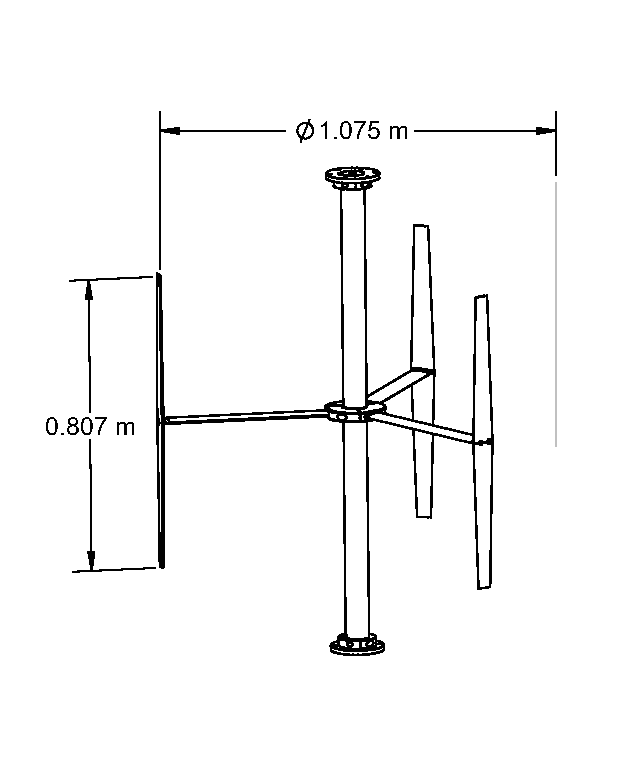
\includegraphics[width=0.65\textwidth]{figures/turbine.eps}

    \caption{{\bf Turbine Model.} A drawing of the turbine model.}

    \label{fig:turbine-drawing}
\end{figure}

The rotor was 1.075 m in diameter and 0.8067 m tall, with blade chords that
taper from 0.04 m at the tips to 0.067 m at the roots, or half-span. Mean
chord-to-radius ratio $c/R$ was 0.1, which is approximately at the threshold
between high and low solidity \cite{Strickland1981,Fiedler2009}. This rotor
geometry presents a unique validation case not yet seen in the literature,
similar in concept to the VAWT 850 \cite{Mays1990} with its tapered blades, but
with a moderately high $c/R$ to more accurately represent typical MHK rotors,
which presents a challenge for numerical modeling.

For investigating the effects of support strut drag losses, a set of cylindrical
covers were designed to slip over the struts, which provided a significant
increase in strut drag. Endcaps were also fabricated to allow the high drag
strut cover configuration to be operated without blades. A drawing of the strut
covers is shown in Fig.~\ref{fig:covers}.

\begin{figure}
    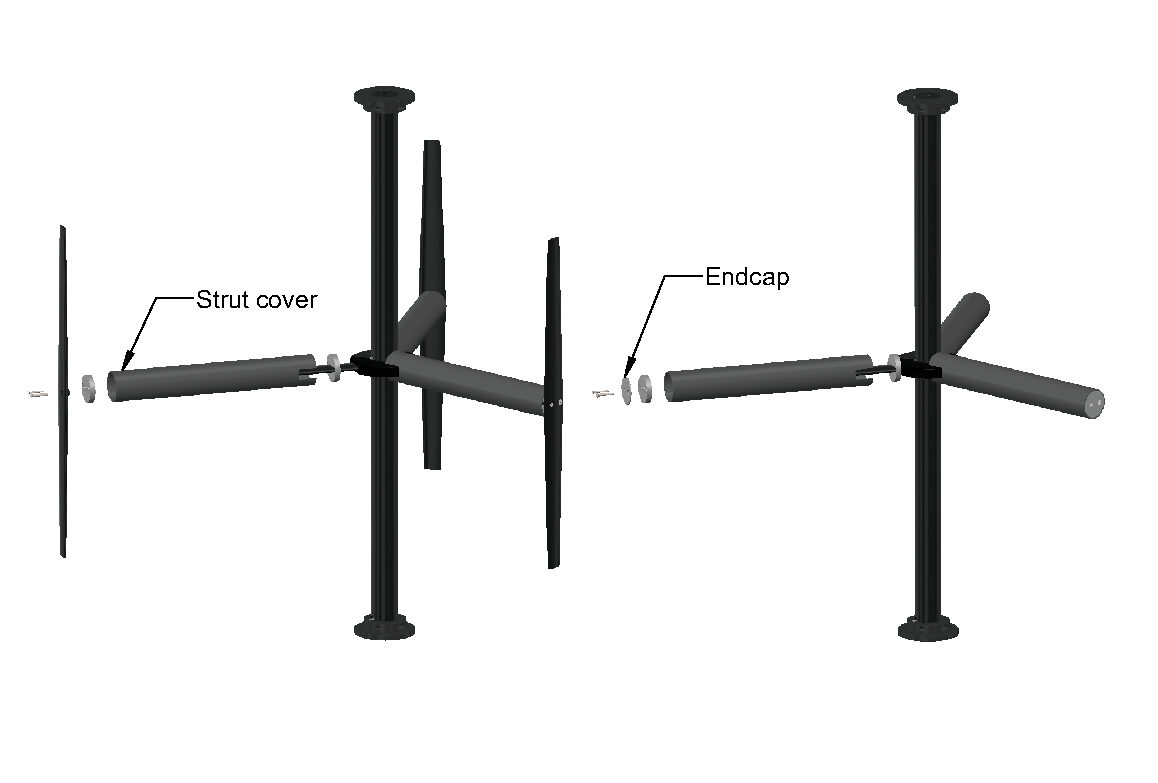
\includegraphics[width=0.95\textwidth]{figures/strut_covers.eps}
    
    \caption{{\bf Strut Covers.} A drawing of the high drag strut cover
        configuration with and without blades.}
    
    \label{fig:covers}
\end{figure}


\subsection*{Facility and instrumentation}

Measurements were conducted in the UNH tow/wave tank, pictured in
Fig.~\ref{fig:exp-setup}, a 36 m long facility with a 3.66 m wide by 2.44 m deep
cross-section, capable of tow speeds up to 3 m/s. The blockage ratio based on
the rotor frontal and tank cross-sectional area was 10\%. The turbine was
mounted in a frame built from NACA 0020 struts, attached to the tow carriage by
four linear bearings, which transfer all streamwise force to a pair of 500 lbf
capacity Sentran ZB3 S-beam load cells \cite{SentranZB}. The turbine shaft RPM
was controlled by a servo motor system, which allowed precise control of the
turbine tip speed ratio. The load torque was measured by an Interface T8 200 Nm
capacity inline rotary torque transducer \cite{InterfaceT8}. An additional
Sentran ZB3 load cell mounted at a fixed distance from the servo motor via a
moment arm provided a redundant torque measurement, measurements from which were
nearly identical to the inline transducer, providing additional confidence in
the results. Turbine shaft angle was measured using the Kollmorgen AKD servo
drive's emulated encoder output \cite{KollmorgenAKD}, set to $10^5$ counts per
turbine shaft revolution. Carriage speed, and therefore inflow velocity was
measured using a Renishaw LM15 linear encoder with 10 $\mu$m resolution
\cite{RenishawLM15}. All of these performance-related quantities were sampled at
2 kHz, while the tow tank's motion controller provided redundant measurements of
the carriage speed turbine angular velocity sampled at 1 kHz. Turbine wake
measurements at 1 meter downstream were measured with a Nortek Vectrino+
acoustic Doppler velocimeter \cite{NortekVectrino}, sampling at 200 Hz. A photo
and drawing of the experimental setup are shown in
Fig.~\ref{fig:exp-setup-photo} and Fig.~\ref{fig:exp-setup}, respectively.

\begin{figure}
    \centering

    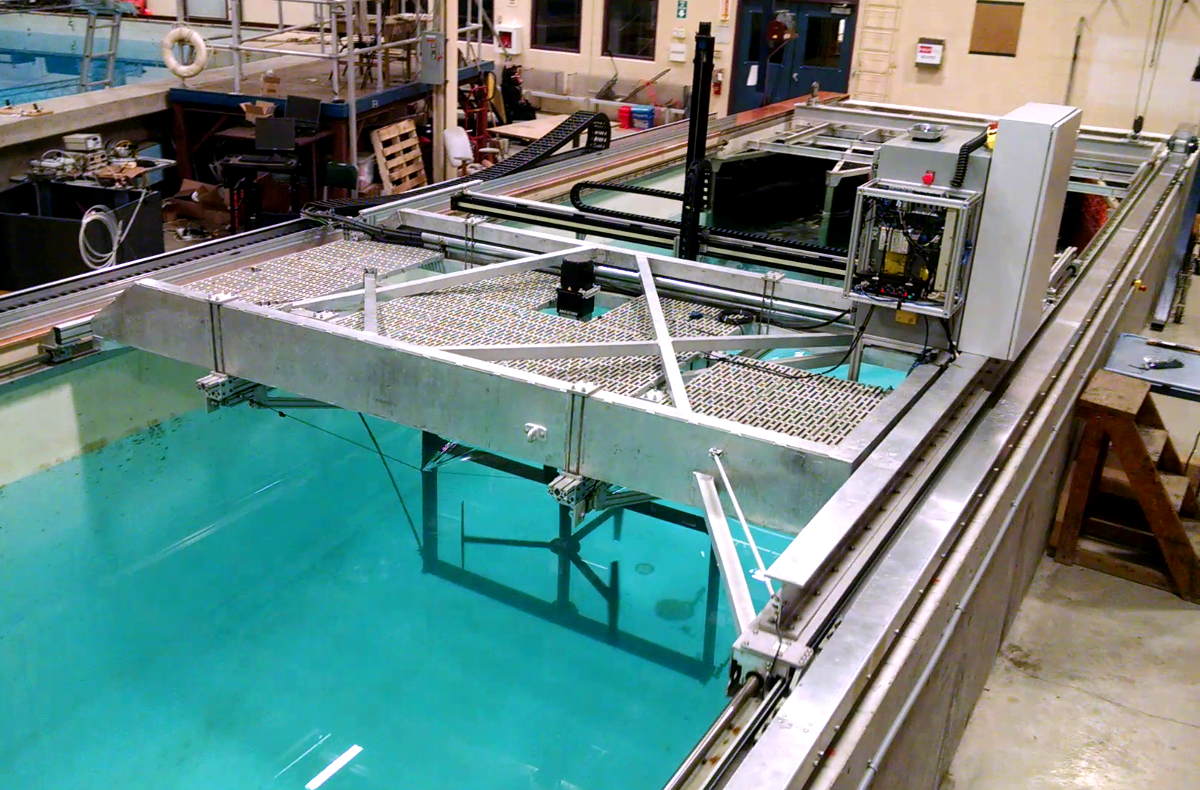
\includegraphics[width=0.95\textwidth]{figures/exp-setup-photo}

    \caption{\textbf{Experimental setup.} Photo of the UNH tow tank and turbine
    test bed with RM2 installed.}

    \label{fig:exp-setup-photo}
\end{figure}

\begin{figure}
    \centering

    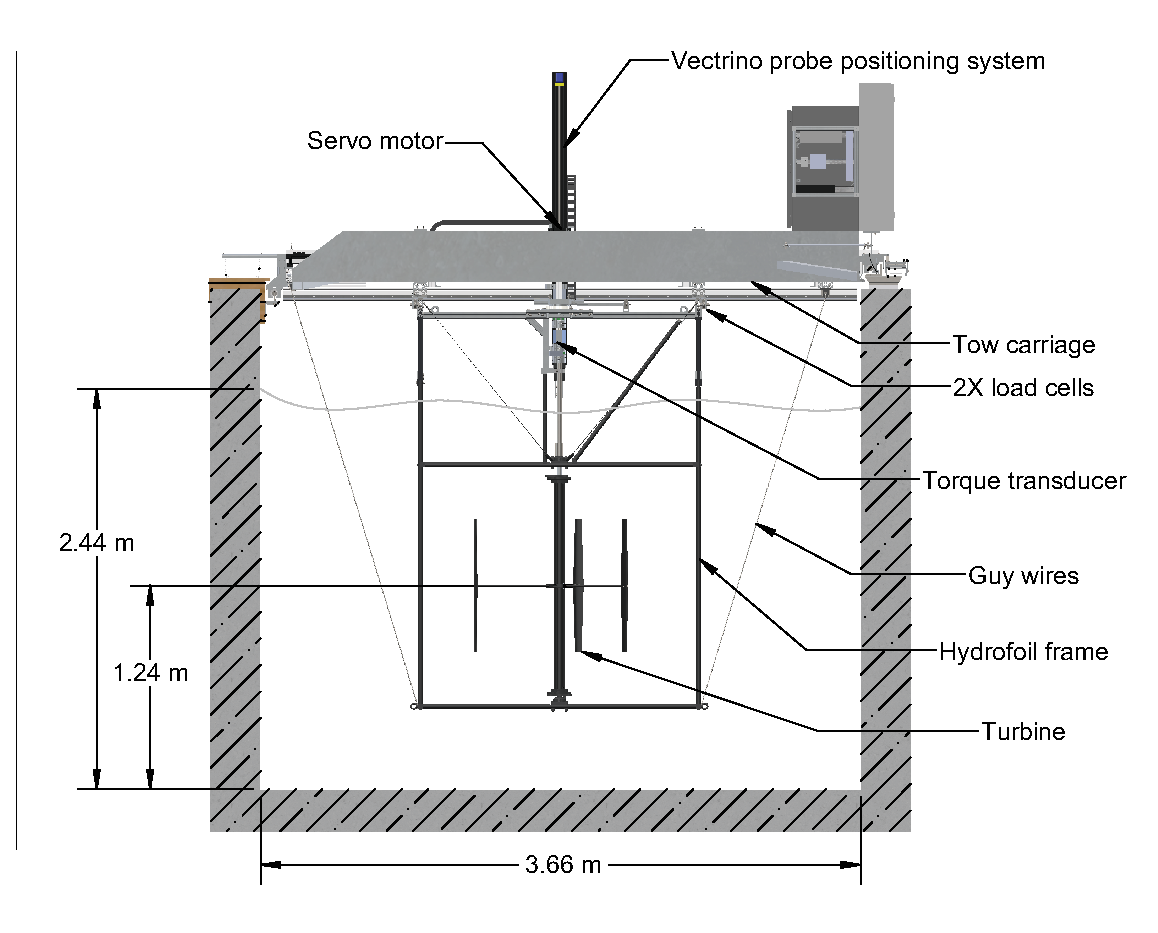
\includegraphics[clip,trim=0.01in 0 0 0,
    width=\textwidth]{figures/tank_cross_section}

    \caption{{\bf Experimental setup.} Illustration of the experimental setup.}

    \label{fig:exp-setup}
\end{figure}


\paragraph{Synchronization.} The three data acquisition instrumentation
subsystems---motion controller, NI DAQ (performance measurements), and Vectrino+
(wake velocity measurements)---started sampling at precisely the same time each
tow, after being triggered by a digital signal edge from the motion controller.
This strategy retained synchronization for all performance signal samples (tow
speed, torque, drag, angular velocity), ensuring precise calculation of, e.g.,
power coefficient. Since there was also synchronization of the initial sample
from each of the three subsystems, correlation of events in the performance and
wake signals is also possible.

\paragraph{Tare drag and torque compensation.} To best estimate the hydrodynamic
loads on the turbine rotor alone, tare torque and drag runs were performed to
measure the shaft bearing friction torque and turbine mounting frame drag,
respectively. Tare drag runs---measured with the turbine removed---were
performed for each tow speed in the experiment, for which the mean value was
subtracted in data processing, to arrive at an estimate for drag on the turbine
alone. Tare torque runs were performed by rotating the turbine shaft (without
blades) in air at constant angular velocity for a specified duration, over the
range of angular velocities used throughout the experiment. Tare torque was fit
with a linear regression versus shaft angular velocity, and added to the
measured turbine torque in post-processing.


\subsection*{Test parameters}

Data collection runs were separated into individual tows, for which all
independent variables---tow speed, tip speed ratio, velocity probe
position---were held constant. These runs were grouped into logical test matrix
``sections,'' in which typically a single independent variable was varied. Test
matrix section names and descriptions are provided in the \texttt{README.md}
file of the experimental data and code repository \cite{Bachant2015-RM2-data}.
Tow speed and their corresponding turbine diameter and blade chord Reynolds
numbers are presented in Tab.~\ref{tab:re}.

\begin{table}
\centering
\begin{tabular}{c|c|c|c|c}
Tow speed (m/s) & $Re_D$ & $Re_{c_\mathrm{tip}}$ & $Re_{c_\mathrm{root}}$ & $Re_{c_\mathrm{mid}}$\\
\hline
0.4 & $4.3 \times 10^5$ & $5.0 \times 10^4$ & $8.3 \times 10^4$ & $6.6 \times 10^4$ \\
0.6 & $6.5 \times 10^5$ & $7.4 \times 10^4$ & $1.2 \times 10^5$ & $9.9 \times 10^4$ \\
0.8 & $8.6 \times 10^5$ & $9.9 \times 10^4$ & $1.7 \times 10^5$ & $1.3 \times 10^5$ \\
1.0 & $1.1 \times 10^6$ & $1.2 \times 10^5$ & $2.1 \times 10^5$ & $1.7 \times 10^5$ \\
1.2 & $1.3 \times 10^6$ & $1.5 \times 10^5$ & $2.5 \times 10^5$ & $2.0 \times 10^5$ \\
\end{tabular}

\caption{{\bf Test Reynolds numbers.} Turbine diameter and approximate average
blade chord Reynolds numbers $Re_c \equiv \lambda U_\infty c / \nu$ at blade
tip, root, and mid-span, corresponding to various tow speeds at $\lambda=3.1$.}

\label{tab:re}
\end{table}

Wake measurements were all performed at 1 m downstream, which corresponds to
$x/D = 0.93$. The cross-stream and vertical coordinates are shown in
Fig.~\ref{fig:coordinates}.

\begin{figure}
    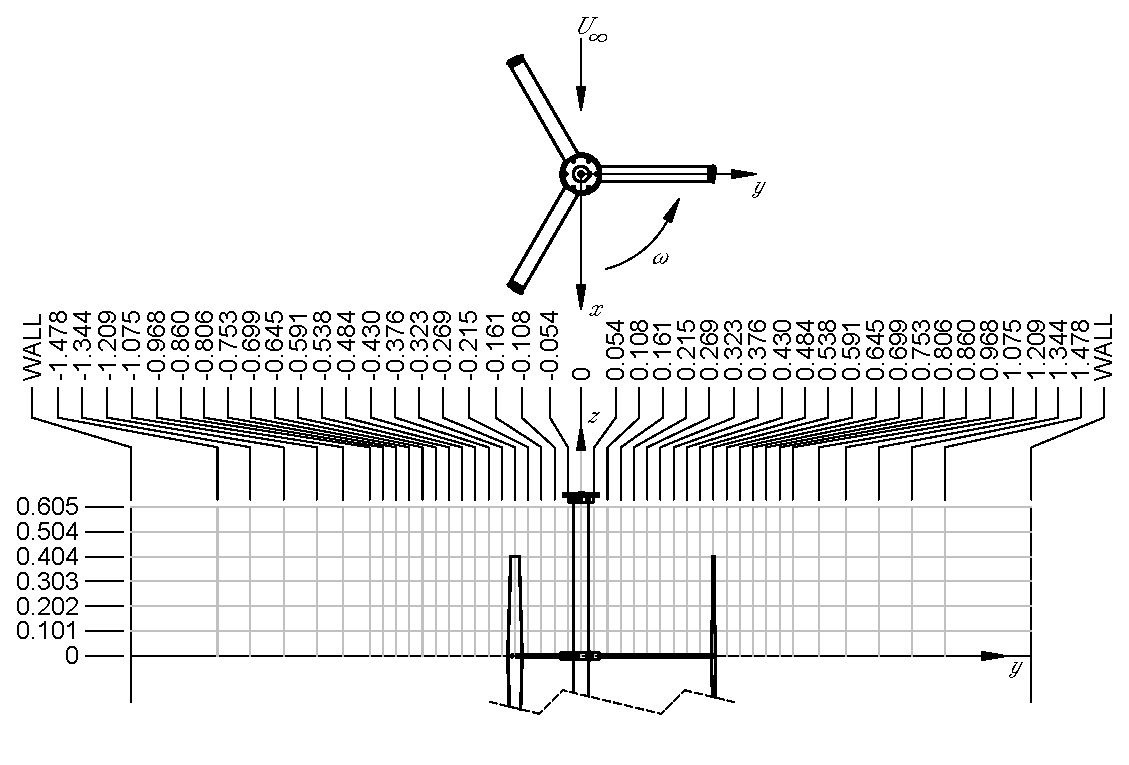
\includegraphics[width=\textwidth]{figures/turbine_coordinate_system.eps}

    \caption{{\bf Coordinate system.} Wake measurement coordinate system and
    cross-stream/vertical coordinates. All dimensions are in meters.}

    \label{fig:coordinates}
\end{figure}


\subsection*{Uncertainty Analysis}

For the mean rotor power and drag coefficients an expanded uncertainty interval
with 95\% confidence
\begin{equation}
    U_{95} = t_{95} u_c,
\end{equation}
was computed, where $t_{95}$ is the value from the Student-$t$ distribution for
a 95\% confidence interval and $u_c$ is the combined standard uncertainty
\cite{ColemanSteele}. Combined standard uncertainty for the sample mean of a
given quantity $X$ is calculated by
\begin{equation}
    u_X^2 = s_{\bar{X}}^2 + b_X^2,
\end{equation}
where $s_{\bar{X}}$ is the sample standard deviation of the mean per turbine
revolution ($s_{\bar{X}} = s_X/\sqrt{N}$), and $b_X$ is the systematic
uncertainty, computed as
\begin{equation}
    b_{X}^2 = \sum_{i=1}^J \left( \frac{\partial X}{\partial x_i} \right)^2
    b_{x_i}^2,
\end{equation}
where $x_i$ is a primitive quantity used to calculate $X$ (e.g. $T$, $\omega$,
and $U_\infty$ for calculating $C_P$), and $b_{x_i}$ is the primitive quantity's
systematic uncertainty, estimated as half the value listed on the sensor
manufacturer's calibration or datasheet.

Selecting $t_{95}$ requires an estimate for degrees of freedom $\nu_X$, which
was obtained using the Welch--Satterthwaite formula
\begin{equation}
    \nu_X = \frac{\left(s_X^2 + \sum_{k=1}^M b_k^2 \right)^2} {s_X^4/\nu_{s_X} +
    \sum_{k=1}^M b_k^4/\nu_{b_k}},
\end{equation}
where $\nu_{s_X}$ is the number of degrees of freedom associated with $s_X$ and
$\nu_{b_k}$ is the number of degrees of freedom associated with $b_k$.
$\nu_{s_X}$ is assumed to be $(N-1)$, where $N$ is the number of independent
samples (or turbine revolutions). The degrees of freedom parameter $\nu_{b_k}$
was estimated as
\begin{equation}
    \nu_{b_k} = \frac{1}{2} \left( \frac{\Delta b_k}{b_k} \right)^{-2},
\end{equation}
where the quantity in parentheses is the relative uncertainty of $b_k$, assumed
to be 0.25.


\subsection*{Data Processing}

For each tow speed, a relevant quasi-steady duration was selected by manually
inspecting a plot of the $C_P$ time series, and then truncated to include a
whole number of blade passages. Over this duration relevant statistics were
calculated. 

Since the blockage ratio was relatively low (10\%), and a definitive blockage
correction for cross-flow turbines has not been established \cite{Cavagnaro2014}
blockage effects were not corrected for. Furthermore, most numerical modeling
efforts can easily incorporate finite domains, meaning blockage corrections
could complicate validation efforts.

To calculate turbine RPM from shaft angle, the encoder signal was differentiated
using a second order central difference scheme, after which an 8 sample wide
moving average smoothing filter was applied to match the noise level present in
the redundant turbine RPM measurement from the motion controller. A similar
approach was used for calculating tow carriage speed $U_\infty$ from carriage
position measurements. Power and drag coefficients are calculated as
instantaneous quantities from the carriage speed as

\begin{equation}
    C_P = \frac{T \omega}{\frac{1}{2} \rho A U_\infty^3}
\end{equation}
and
\begin{equation}
    C_D = \frac{F_\mathrm{drag}}{\frac{1}{2} \rho A U_\infty^2},
\end{equation}
where $\rho$ is the fluid density (1000 kg/m\textsuperscript{3}) and $A$ is
the turbine frontal area $DH$.

All data processing and plotting code, along with the reduced dataset, are
available from \cite{Bachant2015-RM2-data}. Note that this code will
automatically download raw data as necessary so users can perform a full
reanalysis of the measurements presented here.


\section*{Results and Discussion}

\subsection*{Performance}

Mean rotor power coefficients for multiple Reynolds numbers are plotted versus
tip speed ratio in Fig.~\ref{fig:cp-curves}. In general, $C_P$ increases with
$Re$, along with a reduction in the optimal tip speed ratio, due to the tendency
of foils to stall at higher angles of attack at higher $Re$, and the higher
angle of attack ranges seen by the blades at lower $\lambda$. These effects
diminish with increasing $Re$, which is expected as the blade boundary layers
transition to turbulence closer to the leading edge \cite{Lissaman1983,
    McMasters1980, Bachant2016-RVAT-Re-dep}, which helps flow remain attached longer
as it moves against the adverse pressure gradient on the suction side of the
foil. Note how at lower tip speed ratios and Reynolds numbers, $C_P$ becomes
significantly negative, which was possible thanks to the speed control of the
experimental setup's servo motor applying negative torque to the rotor.

\begin{figure}
    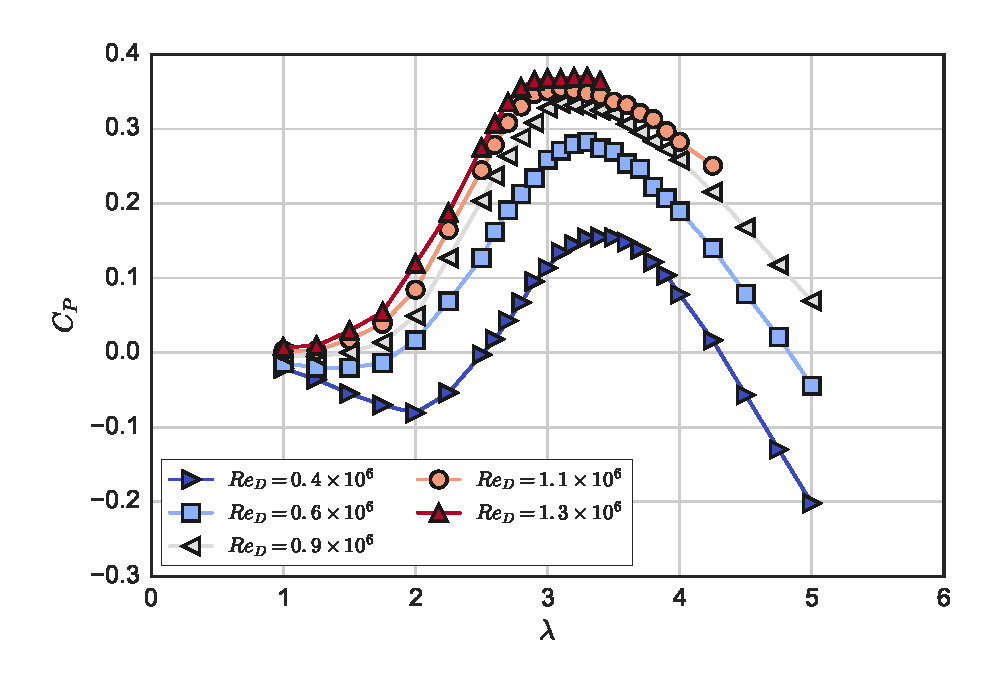
\includegraphics[width=0.9\textwidth]{figures/cp_curves.eps}

    \caption{{\bf Power Coefficient Curves.} Mean rotor power coefficient
    plotted versus mean tip speed ratio for multiple Reynolds numbers.}

    \label{fig:cp-curves}
\end{figure}

Mean rotor drag coefficients are plotted versus tip speed ratio in
Fig.~\ref{fig:cd-curves}. These $C_D$ curves show fewer differences compared to
the power coefficient curves, which is most noticeable at low $\lambda$ and low
$Re$. The relative similarity could be attributed to the effects of stall, where
the lift-to-drag ratio on the blades may drop, decreasing rotor torque, though
the total resultant force due to high blade drag retains a similar component in
the streamwise direction.

\begin{figure}
    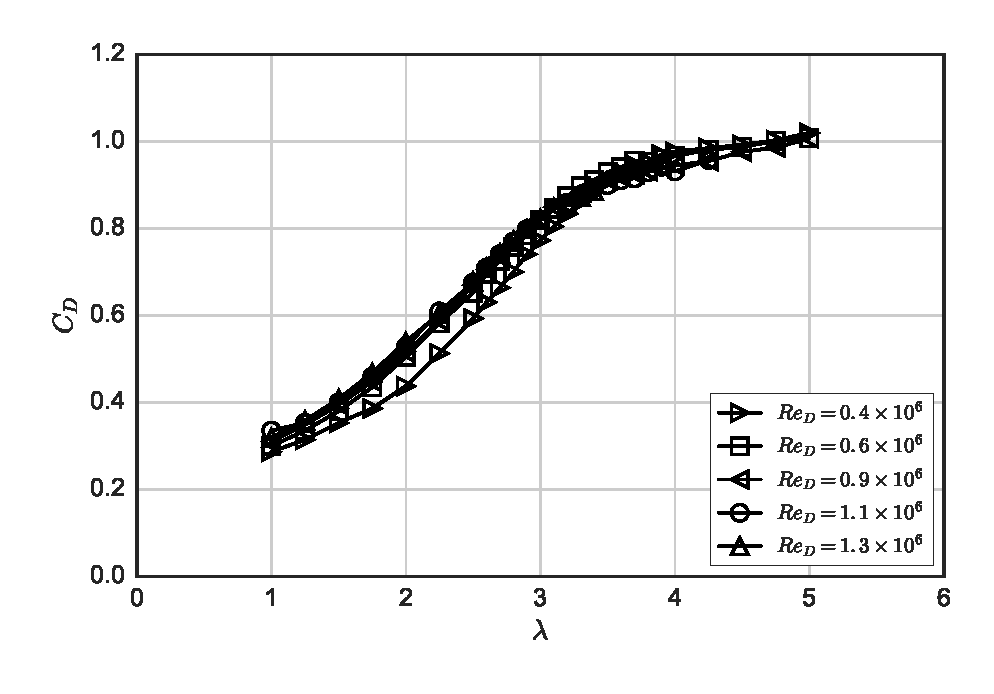
\includegraphics[width=0.9\textwidth]{figures/cd_curves.eps}

    \caption{{\bf Drag Coefficient Curves.} Mean rotor drag coefficient plotted
    versus mean tip speed ratio for multiple Reynolds numbers.}

    \label{fig:cd-curves}
\end{figure}

The power coefficient curves do not collapse exactly onto each other, indicating
Reynolds number dependence, though the differences become relatively small as
$Re$ is increased. Note that the data collection was limited at higher $Re$ and
$\lambda$ due to the unsteady turbine force resonating with the tow carriage
drive belt. However, in contrast to the power coefficient data, the rotor drag
coefficient curves nearly collapse onto each other for $Re_D \ge 0.6 \times
10^6$.

The behavior of the power and drag coefficients at $\lambda=3.1$ are plotted in
Fig.~\ref{fig:perf-re-dep}, where we can see a Reynolds number independent value
of $C_D$ was observed. The power coefficient of the turbine increases
dramatically below $Re_D = 1 \times 10^6$ or $Re_c \equiv \lambda U_\infty c /
\nu \approx 2 \times 10^5$, beyond which there appears to be a small, linear,
positive trend. The tendency of $C_P$ to continue increasing slightly could be
an effect of flow curvature---caused by the finite $c/R$---which imparts a
``virtual camber'' \cite{Migliore1980}, or can be thought of as producing a
``lead'' in angle of attack since cambered airfoils have non-zero lift at zero
angle of attack \cite{Goude2012}. The weaker $Re$-independence of the RM2
compared to that of the higher $c/R$ UNH-RVAT could be due to this virtual
camber effect, since camber has been shown to cause earlier $Re$-convergence of
the CFT's geometric torque coefficient when calculated from static foil
coefficients given by a viscous panel method, whereas characteristics like
lift-to-drag ratio do not converge as strongly \cite{Bachant2016-RVAT-Re-dep}.

\begin{figure}
    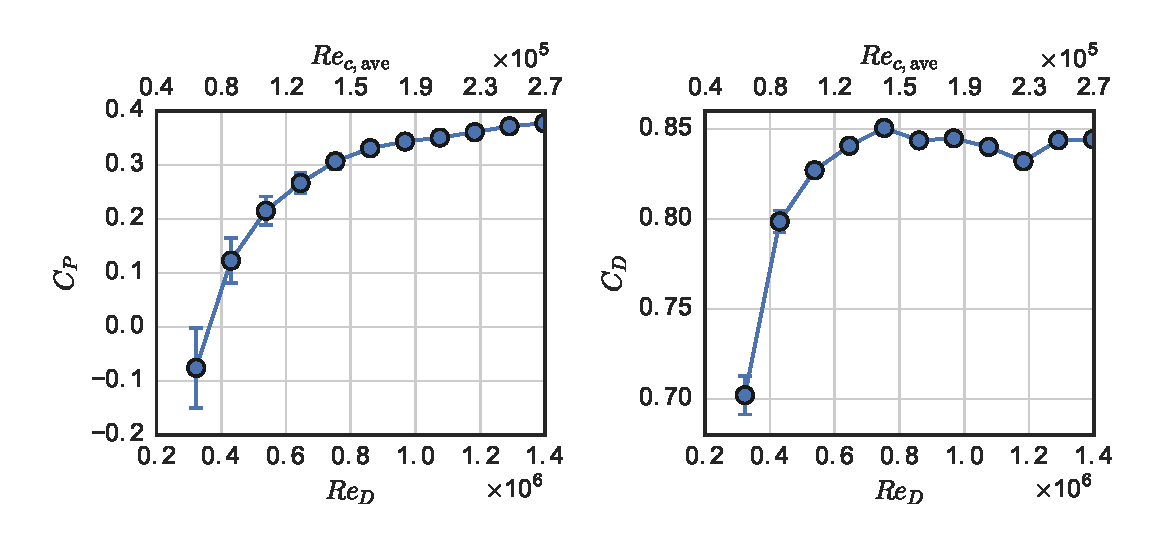
\includegraphics[width=\textwidth]{figures/perf_re_dep.eps}

    \caption{{\bf Reynolds Number effects on performance.} Power and drag
    coefficient at $\lambda=3.1$ plotted versus turbine diameter and approximate
    average blade root chord Reynolds number.}

    \label{fig:perf-re-dep}
\end{figure}


\subsection*{Strut drag losses}

Performance curves for the rotor with both NACA 0021 and cylindrical struts are
shown in Fig.~\ref{fig:perf-covers}. As expected, the high drag cylindrical
struts reduce performance dramatically, which is more pronounced as $\lambda$
increases. This is in accordance with the measurements of Rawlings
\cite{Rawlings2008}, though the strut losses in this case are larger due to the
very high drag profile.

\begin{figure}
    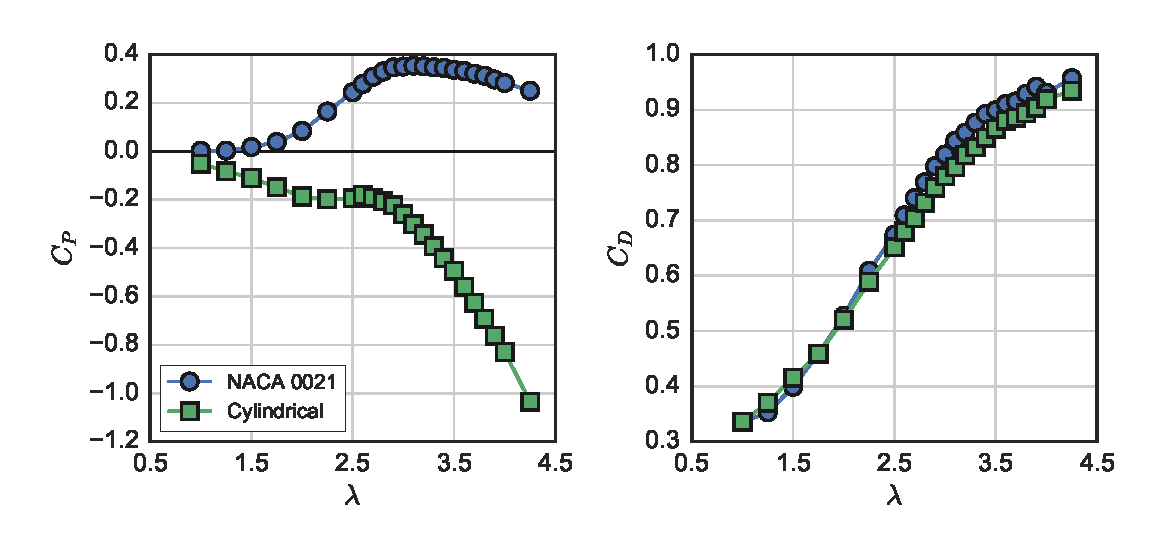
\includegraphics[width=\textwidth]{figures/perf_covers.eps}
    
    \caption{{\bf High drag strut performance.} Turbine performance and rotor
        drag coefficient curves with both NACA 0021 and cylindrical struts.}
    
    \label{fig:perf-covers}
\end{figure}

Measurements for the power coefficient contributions of the strut drag losses
are presented in Fig.~\ref{fig:no-blades} for NACA 0021 and cylindrical
struts---both in towed and stationary conditions. These are computed in the same
fashion as the curves in Fig.~\ref{fig:cp-curves}, but with the blades removed.
We see that strut drag losses increase with tip speed ratio to the power 2--3,
which makes streamlined struts much more important for low solidity turbines,
given the inverse correlation between solidity and $\lambda_0$
\cite{Templin1974}.

\begin{figure}
    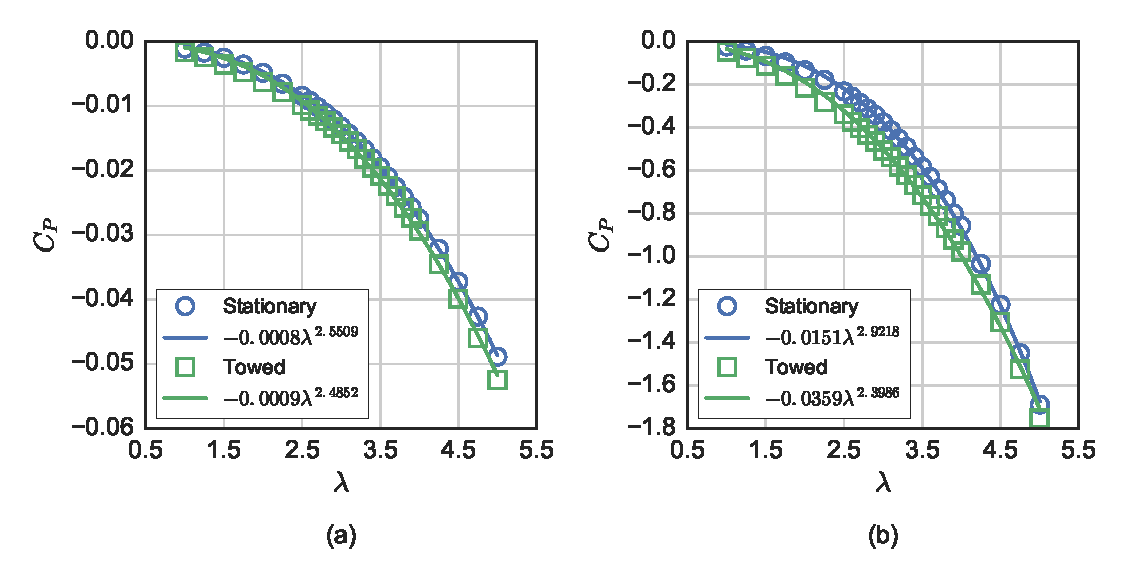
\includegraphics[width=\textwidth]{figures/no_blades_all.eps}
    
    \caption{{\bf Strut drag losses.} Measurements of the strut drag losses for
        (a) NACA 0021 and (b) cylindrical struts, both stationary and towed.}
    
    \label{fig:no-blades}
\end{figure}

Strut drag losses did not change much for the streamlined NACA 0021 struts in
the towed versus stationary configuration, which helps explain why overall rotor
drag coefficients remained relatively constant even at low Reynolds number,
where $C_P$ was dramatically reduced, or even negative. For the cylindrical
struts, losses increased significantly when towed and operating in the mid range
of tip speed ratios. Though a real turbine would never use such high drag
struts, with respect to numerical modeling, these measurements will allow
support struts to be simulated without blades, to isolate and evaluate the
ability to predict these losses independent of the blade loading.


\subsection*{Near-wake characteristics}

The mean velocity field at the chosen optimal tip speed ratio $\lambda_0=3.1$, 1
m downstream ($x/D=0.93$) is plotted in Fig.~\ref{fig:meancontquiv}. The mean
streamwise velocity deficit is markedly more symmetric than that of the
UNH-RVAT, shown in Fig.~\ref{fig:rvat-meancontquiv}, with the RM2 inducing lower
acceleration around the turbine due to the lower rotor drag coefficient and a
slightly lower blockage ratio \cite{Bachant2015-JoT}. Tip vortex shedding is
relatively weaker, which is likely an effect of the RM2's smaller blade chord
length and tapered blades.

\begin{figure}
    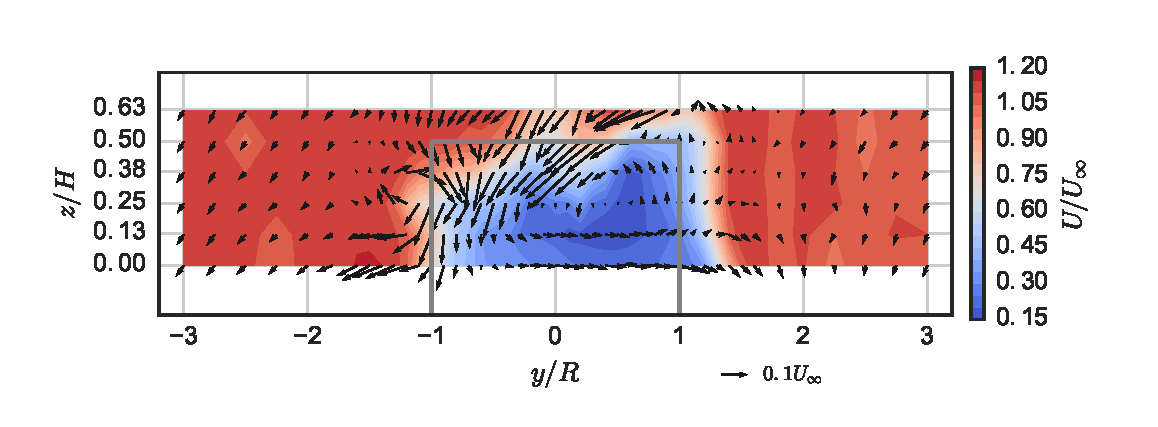
\includegraphics[width=\textwidth]{figures/RVAT-Re-dep-meancontquiv_10.eps}
    
    \caption{{\bf UNH-RVAT Near-Wake Mean Velocity.} UNH-RVAT near-wake mean
        velocity field (looking upstream) at 1 m downstream ($x/D=1.0$),
        $U_\infty=1.0$ m/s, and $\lambda=1.9$, from \cite{Bachant2016-Energies}.
        Solid dark gray lines indicate turbine frontal area.}
    
    \label{fig:rvat-meancontquiv}
\end{figure}

\begin{figure}
    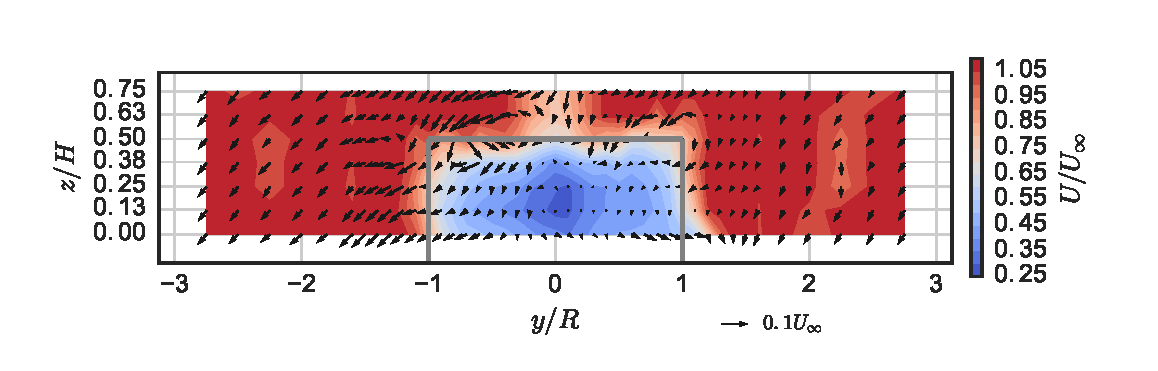
\includegraphics[width=\textwidth]{figures/meancontquiv.eps}

    \caption{{\bf RM2 Near-Wake Mean Velocity.} RM2 near-wake mean velocity
        field (looking upstream) at 1 m downstream ($x/D=0.93$), $U_\infty=1.0$ m/s,
        and $\lambda=3.1$. Refer to Fig.~\ref{fig:coordinates} for turbine axis
        orientation. Solid dark gray lines indicate turbine frontal area.}

    \label{fig:meancontquiv}
\end{figure}

Fig.~\ref{fig:kcont} shows the turbulence kinetic energy in the turbine wake. We
mainly see unsteadiness in the flow generated by the blade tip vortex shedding
(the horizontal band around $z/H=0.5$). Compared with the UNH-RVAT, shown in
Fig.~\ref{fig:rvat-kcont}, turbulence generation is lower overall, without the
intense vertical band around $y/R=-1$, which indicates that the RM2 blades are
operating further from stall---consistent with its higher optimal tip speed
ratio.

\begin{figure}
    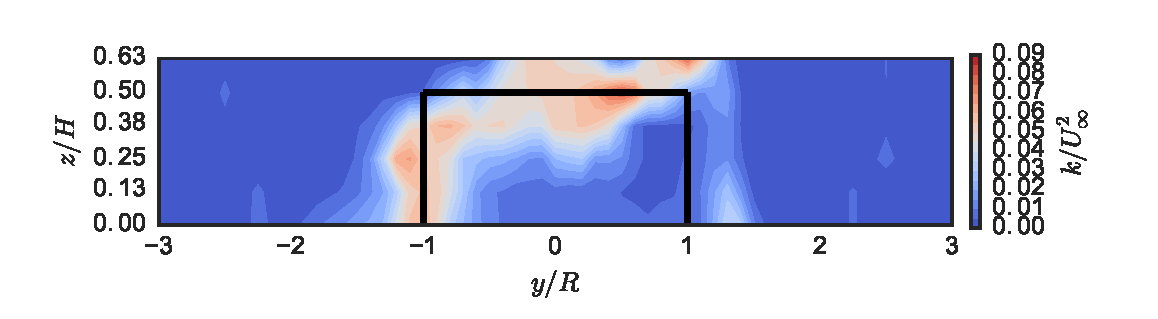
\includegraphics[width=\textwidth]{figures/RVAT-Re-dep-k_contours_10.eps}
    
    \caption{{\bf UNH-RVAT Near-Wake Turbulence Kinetic Energy.} Turbulence
        kinetic energy in the UNH-RVAT's near-wake (looking upstream) at 1 m
        downstream ($x/D=1.0$), $U_\infty=1.0$ m/s, and $\lambda=1.9$, from
        \cite{Bachant2016-Energies}. Solid black lines indicate turbine frontal
        area.}
    
    \label{fig:rvat-kcont}
\end{figure}

\begin{figure}
    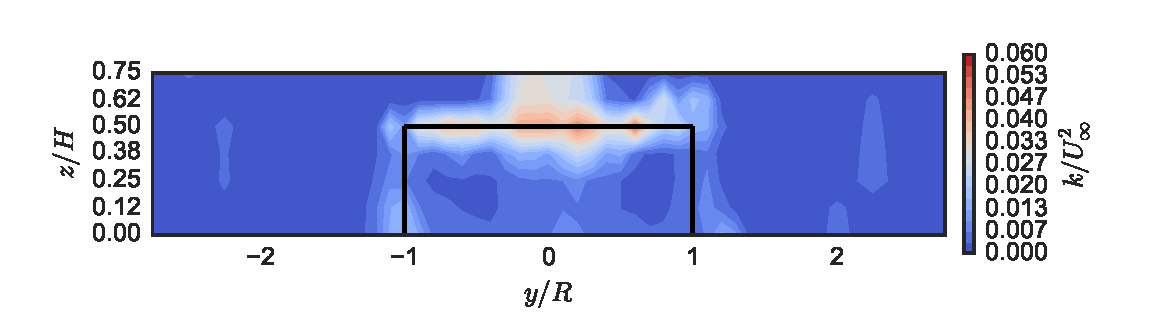
\includegraphics[width=\textwidth]{figures/k_contours.eps}

    \caption{{\bf RM2 Near-Wake Turbulence Kinetic Energy.} Turbulence kinetic
        energy in the RM2's near-wake (looking upstream) at 1 m downstream
        ($x/D=0.93$), $U_\infty=1.0$ m/s, and $\lambda=3.1$. Solid black lines
        indicate turbine frontal area.}

    \label{fig:kcont}
\end{figure}

Analysis of the near-wake of the higher solidity UNH-RVAT turbine revealed that
vertical advection was the largest contributor to streamwise recovery
\cite{Bachant2015-JoT}, a trait which is considered an advantage of cross-flow
over axial-flow rotors in arrays \cite{Kinzel2012}. A similar analysis was
undertaken for the RM2, starting with the transport equation for mean kinetic
energy, rearranged to isolate the streamwise partial derivative (indices follow
the Einsteinian convention):
\begin{equation}
    \begin{split}
        \frac{\p K}{\p x}
        =
        \frac{1}{U}
        \bigg{[}
        & - \underbrace{V \frac{\p K}{\p y}}_{y\text{-adv.}}
        - \underbrace{W \frac{\p K}{\p z}}_{z\text{-adv.}}
        % Pressure work:
        - \frac{1}{\rho}\frac{\p}{\p x_j} P U_i \delta_{ij}
        % Work by viscous forces
        + \frac{\p}{\p x_j} 2 \nu U_i S_{ij}
        % Turbulent transport of K
        - \underbrace{
            \frac{1}{2}\frac{\p}{\p x_j} \overline{u_i' u_j'} U_i
        }_{\text{Turb. trans.}} \\
        % Production of k
        & + 
        \underbrace{
            \overline{u_i' u_j'} \frac{\p U_i}{\p x_j}
        }_{k\text{-prod.}}
        % Mean dissipation
        - 
        \underbrace{
            2 \nu S_{ij}S_{ij}
        }_{\text{Mean diss.}}
        \bigg{]}.
    \end{split}
    \label{eq:K-full}
\end{equation}

Terms that were able to be calculated from the experimental data are those that
do not involve $x$-derivatives, since all wake measurement locations were at a
fixed downstream distance. The available terms are the cross-stream advection
($y$-adv.), vertical advection ($z$-adv.), transport due to turbulent
fluctuations ($y$-turb. and $z$-turb., separated by the direction of the
derivative), production of turbulence kinetic energy ($k$-prod.), and the
dissipation due to the mean velocity gradient (Mean diss.).

Derivatives were computed with a second order central difference scheme for
interior points, and a second order inward-facing scheme for the edges,
identical to \cite{Bachant2015-JoT}. Weighted averages for these computation are
shown in Fig.~\ref{fig:Ktransport}. Due to the weaker blade vortex shedding,
transport due to vertical advection at this point in the wake was approximately
3 times lower than the higher solidity UNH-RVAT. Note that direct comparison is
somewhat invalid, since the total measurement plane area was about 5\% lower for
this experiment. However, the differences observed are beyond this discrepancy.
We also see relatively lower levels of cross-stream turbulent transport due to
the lack of blade stall vortex shedding. These results may have interesting
implications regarding the application of turbines with lower power coefficient
to possibly improve overall array performance through enhanced transport of
kinetic energy from the free stream, though evaluating these trade-offs will
require a detailed analysis of the downstream evolution and turbine--wake
interaction.

\begin{figure}
    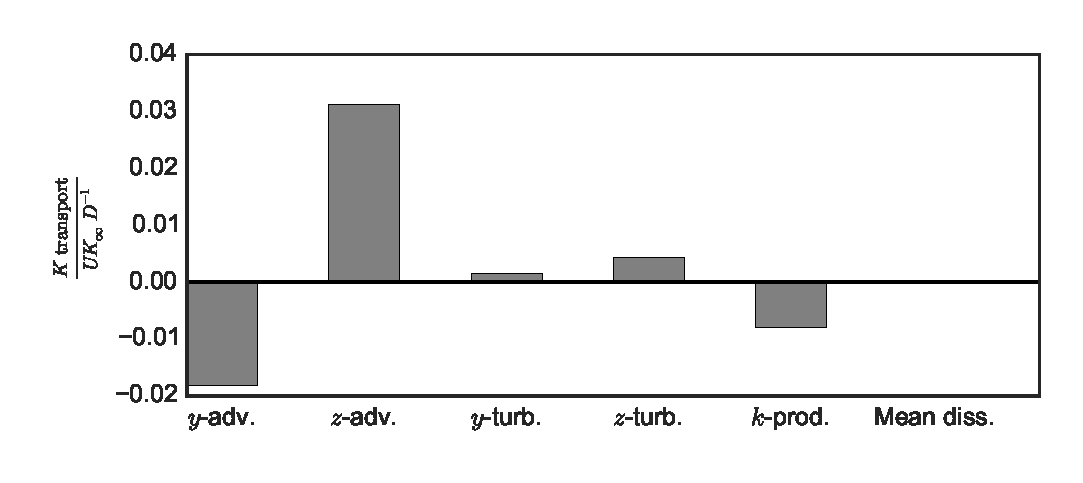
\includegraphics[width=0.9\textwidth]{figures/K_trans_bar_graph.eps}

    \caption{{\bf Mean Kinetic Energy Transport.} Weighted average estimates for
    terms contributing to streamwise recovery of mean kinetic energy, multiplied
    by two due to implied symmetry.}

    \label{fig:Ktransport}
\end{figure}


\subsection*{Conclusions}

The performance and near-wake velocity of a 1:6 scale DOE Reference Model 2
cross-flow turbine was measured in a towing tank. A maximum power coefficient
$C_P = 0.37$ and rotor drag coefficient $C_D = 0.84$ were observed at an optimal
tip speed ratio $\lambda_0 = 3.1$.

Performance was assessed for Reynolds number dependence, showing a convergence
to a weakly $Re$-dependent linear regime at approximately $Re_D \approx 1 \times
10^6$ or $Re_{c,\mathrm{ave}} \approx 2 \times 10^5$. Comparison was made
between this turbine and the higher solidity UNH-RVAT, tested in nearly
identical conditions, which showed similar Reynolds number thresholds but a
flatter linear regime, likely to due virtual camber of the higher
chord-to-radius ratio of the UNH-RVAT blades. Nevertheless, these results
indicate an important transitional scale threshold beyond which data should be
taken for numerical model validation, in order to stay relevant to full scale
devices.

The effects of parasitic drag from blade support struts on turbine performance
were measured by rotating the turbine without blades while stationary and while
towing. These losses---even for a streamlined hydrofoil strut---can become
significant at higher tip speed ratios---up to an approximate 5 percentage point
decrease in power coefficient at a tip speed ratio of 5. These measurements were
repeated with a set of high-drag cylindrical struts, which as expected,
prevented the turbine from producing any mechanical power at any tip speed
ratio. Nevertheless these measurements provide important validation data for
both high and low fidelity numerical performance prediction models, allowing
researchers and engineers to test predictions without blade effects.

While operating at its optimal tip speed ratio $\lambda=3.1$ the wake at
$x/D=0.93$ downstream was shown to be relatively symmetrical and lacked the
evidence of strong blade stall, both of which differentiate this near-wake from
the higher solidity, lower $\lambda_0$ UNH-RVAT. Terms from the mean kinetic
energy transport equation were also computed in this $y$--$z$ plane, showing the
relative importance of the vertical advection compared with turbulent transport
terms at this location, which is qualitatively similar to the UNH-RVAT wake
data. However, lower wake recover totals were calculated. This indicates that
although the RM2 is a more effective energy converter than the UNH-RVAT, its
wake recovery may in fact be delayed due to weaker blade tip vortex shedding and
lower levels of turbulence in the near-wake, which may present a trade-off when
considering optimal array layouts.

This dataset, along with the code for processing and visualization, is provided
openly via a Creative Commons license (MIT license for code), and is available
as a Git repository from \url{http://github.com/UNH-CORE/RM2-tow-tank} or a
citeable archive \cite{Bachant2015-RM2-data}.


\section*{Acknowledgments}

This study was supported by the Department of Energy (DOE), Office of Energy
Efficiency and Renewable Energy (EERE), Wind and Water Power Technologies Office
(WWPTO). Sandia National Laboratories is a multi-program laboratory managed and
operated by Sandia Corporation, a wholly owned subsidiary of Lockheed Martin
Corporation, for the U.S. Department of Energy's National Nuclear Security
Administration under contract DE-AC04-94AL85000.

\nolinenumbers

% Compile your BiBTeX database using our plos2015.bst
% style file and paste the contents of your .bbl file
% here.
%
\bibliographystyle{plos2015}
\bibliography{library}


\end{document}
